\documentclass{article}
\setlength{\oddsidemargin}{0.25 in}
\setlength{\evensidemargin}{-0.25 in}
\setlength{\topmargin}{-0.6 in}
\setlength{\textwidth}{6.5 in}
\setlength{\textheight}{8.5 in}
\setlength{\headsep}{0.75 in}
\setlength{\parindent}{0 in}
\setlength{\parskip}{0.1 in}

% ===== PACKAGES =====
\usepackage{amsmath,amssymb}
\usepackage{color}
\usepackage{subfigure}
\usepackage{graphicx}
\usepackage{mdframed}
\usepackage{changepage}
\usepackage{csquotes}
\usepackage{listings}

\newmdenv[
  topline=false,
  bottomline=false,
  skipabove=\topsep,
  skipbelow=\topsep
]{siderules}
\renewcommand{\abstractname}{}

\usepackage[utf8]{inputenc}
\usepackage{tikz}
\usepackage{minted}
\usetikzlibrary{shadows} % Shadows for nodes

% ===== VARIABLES =====
\def \R{\mathbb{R}}
\def \Pr{\mathbb{P}}
\def \D{{\rm D}}
\def \N{{\rm N}}
\def \xx{{\boldsymbol{\rm x}}}
\def \y{{\rm y}}



% ===== HEADER BOX =====
\newcommand{\lecture}[2]{
\pagestyle{myheadings}
\thispagestyle{plain}
\newpage
\noindent
\begin{center}
\rule{\textwidth}{1.6pt}\vspace*{-\baselineskip}\vspace*{2pt} % Thick horizontal line
\rule{\textwidth}{0.4pt}\\[1\baselineskip] % Thin horizontal line
\vbox{\vspace{2mm}
\hbox to 6.28in { {\bf CS 760: Machine Learning} \hfill Spring 2024 }
\vspace{4mm}
\hbox to 6.28in { {\Large \hfill #1  \hfill} }
\vspace{4mm}
\hbox to 6.28in { {\scshape Authors:}  #2 \hfill }}
\vspace{-2mm}
\rule{\textwidth}{0.4pt}\vspace*{-\baselineskip}\vspace{3.2pt} % Thin horizontal line
\rule{\textwidth}{1.6pt}\\[\baselineskip] % Thick horizontal line
\end{center}
\vspace*{4mm}
}



% =============== DOCUMENT ===============
\begin{document}
\lecture{Graph Neural Networks}{Parla Surendra Mani Kumar}

\begin{center}
\vspace{-0.2in}
{\Large {\sf \underline{\textbf{DO NOT POLLUTE!}} AVOID PRINTING, OR PRINT 2-SIDED MULTIPAGE.}}
\end{center}
\vspace{-0.4in}
\begin{abstract}
Graph Neural Networks (GNNs) are powerful tools for graph-structured data, enabling tasks like node and graph classification, and link prediction. GNNs can capture complex relationships and patterns. We give an overview of GNNs and an abstraction to represent different flavours of GNN like Graph Convolutional Network and Graph Attention Networks. Finally, an example, with code and explanations, is also given.
\end{abstract}
\vspace{-0.2in}
\section{Introduction}

%Neural Networks have been ubiquitous in the areas of pattern recognition, data prediction and crunching knowledge into embeddings. 
Graph Neural Networks (GNN) can be thought as a subset of neural networks which are modelled as graphs. Graphs are non-euclidean data structures where objects are represented as nodes and their relationship is captured as edges. GNN has vast uses cases because there are many datasets which are naturally expressed as graphs, like social media networks, molecules, DNA, internet traffic, knowledge graphs and more.

Historically, Convolutional Neural Networks (CNN) have been highly successful in extracting the spacial features from images and n-D euclidean data structures, but they struggle to capture the relationship present between the nodes as graph can have irregular structures and unequal number of neighbours making convolution operation difficult. 


GNNs can be broadly categorized into 4 types:
\begin{itemize}
    \item Recurrent GNN
    \item Graph Convolutional Neural Networks
    \item Graph Autoencoders (Attension Networks)
    \item Spatial-temporal Graphs (Recursive Networks)
\end{itemize}
\section{Basic Graph Concepts}

\begin{quote}
    A graph G = (V, E) consists of a set of nodes (vertices) V and a set of edges E
\end{quote}
    
%\end{displayquote}

Each edge connects two nodes and represents the relationship between the two nodes. Graphs can be directed (edges have a direction) as shown in Figure \ref{Directed_Graph} (page \pageref{Directed_Graph}) or undirected (edges have no direction) as shown in Figure \ref{Undirected_Graph} (page \pageref{Undirected_Graph}). Additionally, graphs can be weighted, where edges have an associated weight representing the strength of the connection between the nodes. 

%insert image of an undirected and a directed graph

\begin{figure}
     \centering
     \includegraphics[width= 0.4\textwidth]{pics/Directed_Graph.png}
     \caption{Directed Graph}
     \label{Directed_Graph}
\end{figure}

\begin{figure}
     \centering
     \includegraphics[width= 0.4\textwidth]{pics/Undirected_Graph.png}
     \caption{Undirected Graph}
     \label{Undirected_Graph}
\end{figure}

Graphs are represented using the adjacency matrix A where each element in the matrix $A_{ij}$ represent the weight of edge from $node_i$ to $node_j$.

%give the example adjacency matrix for a small graph's node

A degree of node can be defined as the number of neighbour nodes $N(v)$. 

\begin{quote}
    Note : \textit{Nodes} and \textit{edges} are very general terms and can mean a lot of things. For example, a node itself could be a Deep Neural Network and an edge could represent a producer-consumer relationship, evolutionary relationship, a chemical bond, a dataflow relationship or even a mechanical connection.
\end{quote}

\subsection{Modelling Using Graphs}
%\begin{quote}
Graphs allow for the most flexible and accurate representation of a lot of modelling problems. In general, engineering involves the creation of a model with certain (reasonable) assumptions. The objective of creating a model is to ultimately utilise the model for its predictive capabilities. Thus, the modelling framework or approach we take, influences both the way we see a problem and also its solution. A good number of problems that we are trying to solve can be represented as a graph model - 
\begin{enumerate}
    \item Social Media Networks - where every individual is modelled as node and their relation is the edge between them 
    \item Molecules - Every atom is a node and the bond between them is an edge
    \item Proteins - Proteins are represented as a graph (G) of Aminoacids (N) connected to each other by an edge (E)
\end{enumerate}

%\subsection{General Recipe}
So, the basic recipe for a GNN is
\begin{enumerate}
  %\item Identify the graph structure that you want to apply GNN on i.e, formulate the nodes and edges in the data.
  \item Construct the initial graph structure to model the data as nodes and the relationship between data as edges
  \item Based on the task i.e, node level, edge level as described earlier, create the GNN model's classification layer
  \item Define the loss function according to the context. Eg: log likelihood, root mean square error etc.
  \item Apply gradient descent and optimize the weight parameters by minimizing the loss function
\end{enumerate}
%\section{Recurrent GNN - Pritheshwar's task}
Recurrent GNN are the first Graph Neural Networks proposed as early as 2005. 
GNN can categorized in 3 types based on the task:
\subsection{Node-level Task}
In a node level task each node is represented by vector called embedding and the goal here to characterize the node or predict the features if the node. 
Ex: Given a society of individuals predict where a particular person smokes or not 
\subsection{edge level}
In an edge level task the goal is to predict top N possible edges from the interaction in the current graph.
Ex: Recomendation Systems: We have a graph of users and items the task is to recommend new products or videos for the users.
Predicting the time taken to reach a destination in google maps.

\subsection{Graph level}
These tasks involve extracting useful information from the graph.
Ex: Given a molecular structure which is the graph of atoms and bonds predict the aroma of the compund 

Note: AlphaFold 
Google's deepmind has build a model to predict the structure of the protein for a given aminoacids by modeling the interaction to be a Graph Neural Network.
\section{Graph Neural Network}
The function of the graph convolution layer in a GNN is very similar to that of the convolution layer in a CNN, in that the objective is to derive a relationship amongst the nodes. Then, the output from the graph layer is fed into, say, an inference layer for further processing. 
%A Graph Neural Network is very much similar to a 2D convolution neural network with the convolution operation being performed on neighbouring nodes at each layer. 
In supervised learning, we are effectively trying to find a function f(x) which models the output y.
The function $f$, is a neural network which incorporates the graph information.

A GNN layer makes the nodes learn about their neighbours (and all extended neighbours, eventually) over time, by changing each nodes' hidden state. The number of times the hidden state needs to updated is application specific. 

Figure \ref{fgene} (page \pageref{fgene}), shows a real world application of a GNN. It also shows how the GNN layer is separate from the classification layer (FC Layer), as described above.

\begin{figure}
     \centering
     \includegraphics[width= \textwidth]{pics/fgene.jpg}
     \caption{Similarity measure learning of graph neural network in functional brain graphs. The information contained in the fMRI image was integrated into the graph through the graph partition and connection matrix. Two graphs were, respectively, used as the input of the two graph convolutional networks with sharing parameters, and the output of the network was combined by the inner product layer. Finally, a fully connected layer outputs the estimated similarity between the graphs \cite{zhang_graph_2021}}
     \label{fgene}
     %add_ref
\end{figure}

\subsection{Mathematics Behind a GNN}
A single GNN layer consists of two important parts -
\begin{enumerate}
    \item \textbf{Aggregation} - The information from the neighbouring nodes $(N(v))$ us transformed and aggregated. Eg : SUM, MAX, AVERAGE.
    \item \textbf{Update} - The embeddings of the $node (v)$ is updated using the aggregated information from nodes and linearly transformed current node embeddings. Eg : SUM, CONCAT, MLP (Multi Layer Perceptron)
\end{enumerate}

The hidden state of a node at a particular layer $l$ is
\begin{displaymath}
    h_v^{0} = X_v
\end{displaymath}

\begin{displaymath}
    h_v^{(l+1)} = \sigma\Bigl(W_l\sum_{u\in N(v)}\frac{h_u^{(l)}}{|N(v)|} + B_lh_v^{(l)}\Bigr)
\end{displaymath}

The hidden state of all the nodes are transformed using a linear transformation of weight matrix $W_l$ and aggregated using weighted average. 
The current state of the node is also linearly transformed using a weight matrix $B_l$. $\sigma$ is a non linear function, such as the sigmoid function.


\subsection*{Matrix Representation}
Let D be a diagonal matrix where
\begin{displaymath}
   D_{v,v} = Degree(v) = |N(v)|
\end{displaymath}

\begin{displaymath}
    D_{v,v}^{-1} = \frac{1}{|N(v)|}
\end{displaymath}
The term
\begin{displaymath}
    \sum_{u\in N(v)}\frac{h_u^{(l)}}{|N(v)|}
\end{displaymath} 
can be written as
\begin{displaymath}
    D^{-1}AH^{(l)}
\end{displaymath}
Therefore, 
\begin{displaymath}
H^{(l+1)} = \sigma(D^{-1}AH^{(l)}W_l^T + H^{(l)}B_l^T)    
\end{displaymath}

Where $H^{(\ell)}$ is the hidden state matrix at layer $\ell$ and A is the adjacency matrix of the graph. \\ 
The parameters in the weight matrices W and B are tuned by back propagation using MSE (Mean Square Error) or Log Likelihood depending on the ML task.

\begin{displaymath}
\Theta_{\ell,t} = \Theta_{\ell,t-1} - \eta \sum_{i \in \Omega_t} \nabla_i \Theta_{\ell,t-1}    
\end{displaymath}

\subsection{Classification} \label{section_classification}
As a reminder, the GNN layers are used to extract information on how the nodes relate to each other according to our modelling of the problem as a graph. This information is then, commonly, fed into a classification layer.

\begin{figure}
     \centering
     \includegraphics[width= \textwidth]{pics/Classification_Types.jpg}
     \caption{Three Types of GNN Classfication \cite{noauthor_intro_nodate}}
     \label{Classification_Types}
     %add_ref
\end{figure}

Three types of classification exist - 
\begin{enumerate}
    \item Node Classification - here, we try to ascertain what a particular node could be, provided that we have a graph with a good number of nodes labelled
    \item Graph Classification - here, we try to ascertain what the graph as a whole could mean. If we consider an image as a graph, then this would translate to image classification
    \item Link Classification - here, we try to find out if there could be a relationship between two nodes, provided we already have a few links between nodes on the graph
\end{enumerate}

\subsection{General Recipe}
So, the basic recipe for a GNN is
\begin{enumerate}
  %\item Identify the graph structure that you want to apply GNN on i.e, formulate the nodes and edges in the data.
  \item Construct the initial graph structure to model the data as nodes and the relationship between data as edges
  \item Based on the task i.e, node level, edge level as described earlier, create the GNN model's classification layer
  \item Define the loss function according to the context. Eg: log likelihood, root mean square error etc.
  \item Apply gradient descent and optimize the weight parameters by minimizing the loss function
\end{enumerate}
\section{Message Passing GNN}
The message passing GNN layer captures the essence of a GNN. It is the most potent form of a GNN, but it is very expensive to implement - in terms of memory and processing. Thus, they are limited to smaller graphs. 

In message passing GNNs, each node first calculates its message and sends it to its neighbours. Each node then aggregates - the aggregation function depending on the implementation - all the messages that it received from its neighbours. The state of that node is then updated. These happen in lock step across the graph i.e. the state of each node in the graph is updated over time, in each "clock tick". An overview is shown in Figure \ref{Message_Passing_Steps} (page \pageref{Message_Passing_Steps}). 

\begin{quote}
    Note : In certain graph, the edges can be of different types. The edges themselves influence the message that is generated between two nodes
\end{quote}

\begin{figure}
     \centering
     \includegraphics[width= \textwidth]{pics/Message_Passing_Steps.jpg}
     \caption{Dataflow in a Message Passing GNN Layer \cite{noauthor_introduction_nodate}}     \label{Message_Passing_Steps}
     %add_ref
\end{figure}

The change in a node's state can be described using the following equation - 
\begin{displaymath}
 h_t^{n}  = q(h_{t-1}^{n}, {\bigcup_{\forall n_{j} : n_j \xrightarrow{k} n} {f_t(h_{t-1}^{n}, k, h_{t-1}^{n_j}}))
\end{displaymath}

where, $h_t^{n}$ is the state of node $n$ at time $t$. $q$ is a non-linear transformation function. $\bigcup$ is any commutative and permutation invariant operation to combine the messages. $f_t$ is the function that produces the messages according to the previous state of node $n_j$ and node $n$ and edge type $k$. Here, $f_t$ can be dependent on time, but not necessarily.




\section{Graph Convolution Networks}
In a GCN the neighbour embeddings are normalized and summed. These embeddings are then transformed using a weight matrix and a non linear function is applied. See Figure \ref{GCN} (page \pageref{GCN}).
\begin{figure}
     \centering
     \includegraphics[width= 0.6\textwidth]{pics/GNN.png}
     \caption{2D convolution vs Graph Convolution}
     \label{GCN}
     %add_ref
\end{figure}

\begin{displaymath}
    h_u^{(k)} = \sigma \left( W^{(k)} \sum_{v \in N(u) \cup \{u\}} \frac{h_v}{\sqrt{|N(u)||N(v)|}}\right)
\end{displaymath}

This can be expressed in matrix representation as
\begin{displaymath}
    x*_{G} g{\theta} =\theta(I_{n}+D^{-\frac{1}{2}}AD^{-\frac{1}{2}})x
\end{displaymath}
where D is diagonal degree matrix, A is adjacency matrix and x is the input

An example of nodes in a graph and their adjacency matrix is shown in Figure \ref{example_graph} (page \pageref{example_graph}).

\begin{displaymath}
    A = {\begin{bmatrix}
0 & 1 & 1\\
0 & 0 & 1\\
0 & 0 & 0
\end{bmatrix}}, N = {\begin{bmatrix}
    a \\ b \\c
\end{bmatrix}}, A^T.N = {\begin{bmatrix}
    0 \\ a \\ a+b
\end{bmatrix}}
\end{displaymath}

\begin{figure}
    \centering

\begin{tikzpicture}
\tikzset{% This is the style settings for nodes
    dep/.style={circle,minimum size=1cm,fill=orange!20,draw=orange,
                general shadow={fill=gray!60,shadow xshift=1pt,shadow yshift=-1pt}},
    cli/.style={circle,minimum size=1cm,fill=white,draw,
                general shadow={fill=gray!60,shadow xshift=1pt,shadow yshift=-1pt}},
    spl/.style={cli,append after command={
                  node[circle,draw,dotted,
                       minimum size=1.5cm] at (\tikzlastnode.center) {}}},
    c1/.style={-stealth,very thick,red!80!black},
    v2/.style={-stealth,very thick,yellow!65!black},
    v4/.style={-stealth,very thick,purple!70!black}}
\node[cli] (0) at (0,0) {a};
\node[cli] (1) at (-1,-2) {b};
\node[cli] (2) at (2,-2) {c};
%\draw[c1] (0) to[bend right] (7);
\draw[v4] (0) -- (1);
\draw[v4] (0) -- (2);
\draw[v4] (1) -- (2);
\end{tikzpicture}


    \caption{Example Graph}
    \label{example_graph}
\end{figure}


\section{Other Flavours of GNN}


\subsection{GraphSage}
GraphSage proposes the use of different aggregating functions like weigthed avegage, Multi Layer Perceptron on all the neighbouring nodes or even a LSTM.

The aggregated messsages are then concatenated with the node embeddings.
\begin{displaymath}
    m_N^{(u)} = \text{MLP}{\theta} \left( \sum{v \in N(u)} \text{MLP}_{\phi}(h_v)\right)
\end{displaymath}
Other interesting idea here is $\ell_2$ normalization of hidden state in all the layer which seems to improve performance.

\begin{displaymath}
    h_v^{(\ell)} = \frac{h_v^{(\ell)}}{||h_v^{(\ell)}||}_2 \quad where, \quad ||u||_2 = \sqrt{\sum_i u_i^2}
\end{displaymath}

\subsection{Graph Attention Networks}
The aggregate function in the GAT is attention operation. All the neighbouring node embeddings are multiplied by weights i.e, attention coefficients. Comparing this to other flavours where this weight is just the inverse of the degree of the node, attention which is learnt from the network is great replacement for this weight.
\begin{displaymath}
m_v^{(u)} = \sum_{v \in N(u)} \alpha_{u,v} h_v,  \quad \alpha_{u,v} = \frac{\exp(a^T [Wh_u \oplus Wh_v])}{\sum_{v' \in N(u)} {\exp(a^T [W{h_u} \oplus Wh_{v'}])}}
\end{displaymath}

Where a is linear transformation matrix and the operation $\oplus$ can either be concatenation or a dot product or some distance metric like cosine similarity.

%\section{Future Work}
\section{Over-Smoothing Problem}
Unlike CNN where the performance increase along with the number of layers, GNN with many layers perform poorly. In a highly connected graph network every node is influenced by many neighbours. So, with huge number of layers all the node embeddings will be saturated and become indistinguishable to each other. This is called over smoothing effect. The number layers to reach this saturation in a highly connected graph could be as low as O($\log(|v|)$)\\

So, the solution for this problem is instead of increasing the number of GNN layers (k) we can add complexity in the aggregation function with the use of Multi Layer Perceptron (MLP) as in Graph Sage model. This would help you aggregate the spacial information with fewer GNN layers. 
%\subsection{General Recipe}
So, the basic recipe for a GNN is
\begin{enumerate}
  %\item Identify the graph structure that you want to apply GNN on i.e, formulate the nodes and edges in the data.
  \item Construct the initial graph structure to model the data as nodes and the relationship between data as edges
  \item Based on the task i.e, node level, edge level as described earlier, create the GNN model's classification layer
  \item Define the loss function according to the context. Eg: log likelihood, root mean square error etc.
  \item Apply gradient descent and optimize the weight parameters by minimizing the loss function
\end{enumerate}
\section{Example}
We shall now look at an example, with explanations and code.
\begin{quote}
    \textbf{Objective :} To find the solubility of a molecule in a solvent. 
\end{quote}
We will be using the MoleculeNet \cite{noauthor_torch_geometricdatasets_nodate} dataset's ESOL dataset. 
\begin{quote}
    "ESOL is a small dataset consisting of water solubility data for 1128 compounds. The dataset has been used to train models that estimate solubility directly from chemical structures (as encoded in SMILES strings)."
\end{quote}
\begin{figure}
     \centering
     \includegraphics[width= 0.4\textwidth]{pics/smile.png}
     \caption{Smile String of Ibuprofen}
     \label{Smile}
     %add_ref
\end{figure}
Each molecule is represented as a graph, with the nodes representing the atoms. Each node (atom) has a feature vector associated with it. Since the molecule itself is represented as a graph and we would like to find the solubility of the molecule, we are naturally going to make graph level predictions. The GNN architectures vary for different levels of predictions (see section \ref{section_classification}). 

\begin{quote}
    Since this is a graph level task a Pooling layer combines the node representations of the graph into one representation so that every graph is converted to a vector embedding.
\end{quote}

3 simple GCN layers were applied followed by global Max and global Mean pooling of the graph concatenated. 

See Appendix in page \pageref{appsrccode} for some example code.
\nocite{*}
\bibliographystyle{IEEEtran}
\bibliography{IEEEabrv, Library}
%\section{Appendix}
\appendix
\begin{center}
    \Large \textbf{Appendix}
\end{center}
\label{appsrccode}
\inputminted[breaklines]{python}{code.py}
\end{document} 

